\Transcb{yellow}{blue}{Source Strength and Fluxes}
\onecolumn
\begin{itemize}
\item[] \begin{center} {\red Some definitions} \end{center}
\item[] {\blue Source Luminosity ($L$) : Total emitted amount of radiation per unit of time}
\item[] {\blue Flux ($F$) : Amount of radiation passing per unit area per unit of time}
\item[$\ast$] Note : Radiation can represent energy as well as number of particles
\item[$\ast$] Redshift effects are neglected and will be discussed later in this lecture series
\item[] \begin{center} {\red Flux measurements} \end{center}
\item Consider a spherical source with radius $R_{s}$ and luminosity $L$\\
      that radiates photons isotropically from its surface (e.g. a star)
\item Consider a sphere with radius $r>R_{s}$ with the source at its center
\item[] $\rightarrow$ Photon flux at the surface of this sphere: $\displaystyle F=\frac{L}{4\pi r^{2}}$
\item Imagine a detector at some distance $d>R_{s}$ from the center of the source
\item[] $\rightarrow$ Observed flux $F$ will decrease as $d^{-2}$
\item[] {\blue If distance unknown $\rightarrow L$ can not be determined from the observed flux}
\end{itemize}

\Tr
\onecolumn
\begin{itemize}
\item[] \begin{center} {\red What can we infer about the source strength if the distance is not known ?} \end{center}
\item Surface area on a sphere with radius $r$ : $\d A=r^{2} \sin(\theta) \d\theta \d\phi$
\item[] {\blue Solid angle : $\d\Omega \equiv \sin(\theta)\d\theta \d\phi$} which yields {\blue $\d A=r^{2}\d\Omega$}
\item At a distance $d \gg R_{s}$ the source covers a solid angle
      $\displaystyle \Omega_{s}=\int \d\Omega \approx \frac{\pi R_{S}^{2}}{d^{2}}$ sr
\item[] $\rightarrow$ Flux received from a unit of solid angle :
        $\displaystyle \Phi=\frac{F}{\Omega_{s}}=\frac{L}{4\pi (\pi R_{S}^{2})}$
\item[] {\red This does not depend on the distance from the source !}
\item[] $\rightarrow$ Good observable to characterize the source strength
\item No distance dependence $\rightarrow$ Same value at the radiating source
\item[] As seen from the source : $\Phi=$ Flux emitted within a unit of solid angle
\item[] \begin{center} {\blue Source Intensity ($I$) : Flux received c.q. emitted per unit of solid angle} \end{center}
\item[$\ast$] For an extended source that can be resolved, intensity measurements allow to characterize
                     the brightness of different source areas
\end{itemize}

\Tr
\onecolumn
\begin{itemize}
\item[] \begin{center} {\blue How to measure the source intensity ?} \end{center}
\item Consider a detector with area $A$ cm$^{2}$ aimed at a source
\item[] In a time interval $\Delta T$ seconds the detector records $N$ photons\\
        and a deposited energy of $E$ GeV
\item[] Seen from the detector the source spans a circle with radius $\alpha \ll 1$ radians
\item[] $\displaystyle \rightarrow \Omega_{s}=\int_{0}^{\alpha}\sin(\theta)\, \d\theta\int_{0}^{2\pi}\d\phi
         \approx 2\pi\int_{0}^{\alpha} \theta\,\d\theta=\pi\alpha^{2}$
\item[] {\blue Photons : $\displaystyle F=\frac{N}{A\,\Delta T}$ ph cm$^{-2}$ s$^{-1} \quad$
         $\displaystyle I=\frac{N}{A\,\Delta T\,\pi\alpha^{2}}$ ph cm$^{-2}$ s$^{-1}$ sr$^{-1}$}
\item[] {\blue Energy : $\displaystyle F=\frac{E}{A\,\Delta T}$ GeV cm$^{-2}$ s$^{-1} \quad$
         $\displaystyle I=\frac{E}{A\,\Delta T\,\pi\alpha^{2}}$ GeV cm$^{-2}$ s$^{-1}$ sr$^{-1}$}
\item[$\ast$] For (short) transient events one often denotes the {\blue Fluence}
\item[] \begin{center} {\blue Fluence (S) : Time integrated flux} \end{center}
\item[] $\rightarrow$ {\blue $\displaystyle \quad S=\frac{N}{A}$ ph cm$^{-2}$
        $\qquad \displaystyle S=\frac{E}{A}$ GeV cm$^{-2}$}
\end{itemize}

\Tr
\onecolumn
\begin{itemize}
\item In case the detector area $A$ is mis-aligned w.r.t. the incident radiation
\item[] $\rightarrow$ {\blue $A$ has to be replaced by $A\cos(\psi)$}
\end{itemize}
%
\begin{center}
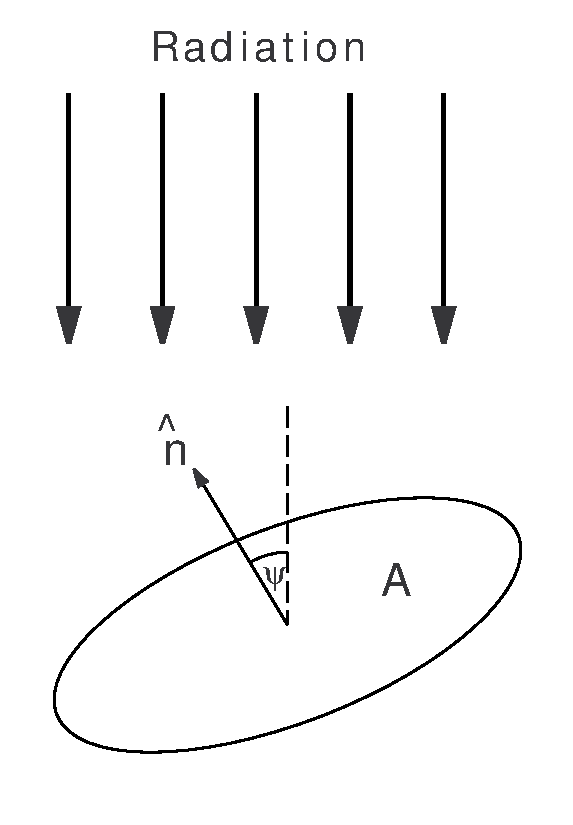
\includegraphics[keepaspectratio,height=11cm]{area}
\end{center}
\begin{itemize}
\item The same holds for the emission when the source area is mis-aligned
\end{itemize}

\Tr
\onecolumn
\begin{itemize}
\item Very often not every incident particle will be recorded by the detector
\item[] This is accounted for by replacing $A$ with the so called {\blue Effective Area $(A_{eff})$}
\item[] {\blue Particles :
        $\displaystyle A_{eff}=\frac{\text{Observed count rate}}{\text{Incoming flux}} =
         \frac{\text{\# Observed counts}}{\text{Incoming fluence}}$}
\item[] {\blue Energy :
        $\displaystyle A_{eff}=\frac{\text{Recorded power}}{\text{Incoming flux}} =
         \frac{\text{Recorded energy}}{\text{Incoming fluence}}$}
\item[$\ast$] $A_{eff}$ can only be determined by simulations or a calibration source
\item[] \begin{center} {\red Flux densities $F(\nu)$ and $F(E)$} \end{center}
\item[] {\blue $F(\nu)\,\d\nu \equiv$ Flux in the frequency interval $[\nu,\nu+\d\nu]$}
\item[] {\blue $F(E)\,\d E \equiv$ Flux in the energy interval $[E,E+\d E]$}
\item[] $\rightarrow$ This leads also to $I(\nu)$, $S(\nu)$, $I(E), S(E)$ etc.
\item[$\ast$] One often uses the notation $F_{\nu}$, $I_{\nu}$, $S_{\nu}$ etc.
\item[] \begin{center}{\blue Special flux density unit : Jansky (Jy)}\end{center}
\item[] {\blue 1 Jy $=10^{-26}$ J s$^{-1}$ m$^{-2}$ Hz$^{-1}
         =10^{-23}$ erg s$^{-1}$ cm$^{-2}$ Hz$^{-1}$}
\item[] {\blue $\qquad =6.25 \cdot 10^{-21}$ GeV s$^{-1}$ cm$^{-2}$ Hz$^{-1}$}
\end{itemize}
